% Complete English translation of the specified Chapter 4 attachment.
% Source numbering and inconsistencies intentionally preserved; see REVIEW-NOTES.md.
\section{Experimental Results and Analysis}
We evaluate the proposed method through three research questions (RQs) concerning known-class recognition, unknown-class rejection, and component contributions:
\begin{itemize}
\item \textbf{RQ1: Does the proposed method offer advantages in known-class recognition?}
\item \textbf{RQ2: Can the proposed method effectively identify and reject unknown services and attacks?}
\item \textbf{RQ3: Do the individual views and the empirical support mechanism contribute to rejection performance?}
\end{itemize}
We design corresponding experiments to address these questions. For RQ1, Section~4.2 compares known-class recognition against existing methods on tasks derived from ISCX-VPN, ISCX-Tor, and other datasets at different class granularities. For RQ2, Section~4.3 evaluates rejection of unknown services and attacks through complete-service holdout on VNAT, class holdout on USTC-TFC2016, and unknown-attack detection on CIC-IDS2017. Section~4.5 further examines the effects of the rejection threshold and changes in the proportion and composition of unknown classes. For RQ3, Section~4.4 compares rejection scores on identical frozen representations and conducts view ablations to assess the contributions of local empirical support and individual view branches.

\subsection{Experimental Setup}
\subsubsection{Datasets and Task Splits}
We use bidirectional flows as samples and evaluate on ISCX-VPN, ISCX-Tor, USTC-TFC2016, CIC-IDS2017, and VNAT.

ISCX-VPN and ISCX-Tor retain six and seven original service labels for the main closed-set comparison. USTC-TFC2016 supplies three class-holdout settings. CIC-IDS2017 supports both known-class classification and unknown-attack diagnosis. VNAT supplies four service-level holdout folds. Table~4-1 lists the class and ID mappings for USTC-TFC2016, ISCX-VPN, and ISCX-Tor; Table~4-2 specifies the USTC and coarse-service class splits.

\begin{table*}[!t]
\centering
\begingroup
\renewcommand{\thetable}{4-1}
\caption{Class and ID mappings for USTC-TFC2016, ISCX-VPN, and ISCX-Tor}\label{tab:source-1}
\fontsize{8}{9.5}\selectfont
\setlength{\tabcolsep}{3pt}
\begin{tabular*}{\textwidth}{@{\extracolsep{\fill}}*{10}{c}@{}}
\hline
ID & Class & ID & Class & ID & Class & ID & Class & ID & Class \\
\hline
U0 & Gmail & U7 & SMB & U14 & MySQL & V0 & Chat & T0 & Chat \\
U1 & FTP & U8 & BitTorrent & U15 & Htbot & V1 & Email & T1 & Email \\
U2 & Nsis-ay & U9 & WorldOfWarcraft & U16 & Tinba & V2 & File Transfer & T2 & File Transfer \\
U3 & Facetime & U10 & Shifu & U17 & Skype & V3 & P2P & T3 & P2P \\
U4 & Weibo & U11 & Outlook & U18 & Miuref & V4 & Streaming & T4 & Audio-streaming \\
U5 & Cridex & U12 & Virut & U19 & Neris & V5 & VoIP & T5 & Video-streaming \\
U6 & Zeus & U13 & Geodo & --- & --- & --- & --- & T6 & VoIP \\
\hline
\end{tabular*}
\par\smallskip\parbox{\textwidth}{\fontsize{7}{8}\selectfont Note: U denotes USTC-TFC2016, V denotes ISCX-VPN, and T denotes ISCX-Tor.}
\endgroup
\end{table*}

\begin{table*}[!t]
\centering
\begingroup
\renewcommand{\thetable}{4-2}
\caption{Experimental scenarios and known/unknown class splits}\label{tab:source-2}
\footnotesize
\setlength{\tabcolsep}{4pt}
\resizebox{\textwidth}{!}{%
\begin{tabular}{lcc}
\hline
Scenario & Known Classes (KC) & Unknown Classes (UC) \\
\hline
A-1 & USTC-TFC2016 \textbackslash{} \{U16\} & U16 (Tinba) \\
A-2 & USTC-TFC2016 \textbackslash{} \{U13, U15, U16\} & U13 (Geodo), U15 (Htbot), U16 (Tinba) \\
A-3 & USTC-TFC2016 \textbackslash{} \{U13, U15, U16, U18, U19\} & U13 (Geodo), U15 (Htbot), U16 (Tinba), U18 (Miuref), U19 (Neris) \\
VPN-4C & \{V0+V1+V5, V2, V3, V4\} & None (closed-set) \\
Tor-5C & \{T0+T1+T6, T2, T3, T4, T5\} & None (closed-set) \\
\hline
\end{tabular}}
\endgroup
\end{table*}

\begin{table}[!t]
\centering
\begingroup
\renewcommand{\thetable}{4-3}
\caption{Sample composition for VNAT complete-service holdout}\label{tab:source-3}
\fontsize{8}{9.5}\selectfont
\setlength{\tabcolsep}{3pt}
\begin{tabular}{@{}ccc@{}}
\hline
Held-out unknown service & Known flows & Unknown flows \\
\hline
Communication & 21,241 & 2,208 \\
File Transfer & 17,579 & 5,870 \\
Remote Access & 9,842 & 13,607 \\
Streaming & 21,685 & 1,764 \\
\hline
\end{tabular}
\endgroup
\end{table}

\setcounter{subsubsection}{1}
\subsubsection{Baselines}
We compare representative encrypted-traffic recognition methods covering closed-set classification and unknown-class detection.
\begin{itemize}
\item \textbf{TrafficFormer} \bluecite{ch2-2}: a pretrained Transformer for encrypted-traffic representation.
\item \textbf{YaTC} \bluecite{ch2-4}: a masked-autoencoder traffic Transformer with multilevel flow representations.
\item \textbf{Open-Detect} \bluecite{ch2-15}: a variational model with Gaussian class prototypes. Its native minimum posterior-to-prototype KL score serves as the VNAT open-set baseline; the closed-set table uses the recorded corrected-paper implementation.
\item \textbf{RoNeTC} \bluecite{ch2-16}: multiview feature extraction and uncertainty-aware traffic classification. The closed-set experiment uses a runnable reconstruction.
\item \textbf{TFE-GNN} \bluecite{ch2-6}: a graph-based traffic encoder. The recorded comparison adapts it to UDP and short flows using up to eight packets.
\item \textbf{Trident} \bluecite{ch2-13}: class-specific one-class learners. The recorded closed-set adaptation uses 86 statistical features from up to eight packets.
\item \textbf{MSP} \bluecite{ch2-17}: negative maximum softmax confidence, used as an unknown score.
\item \textbf{Energy} \bluecite{ch2-18}: an energy score computed from classifier logits.
\end{itemize}
DES-v0 and DES-v1 are the proposed method's centroid-only and centroid-plus-neighbor rejection rules, respectively; Section~III defines them.

\subsubsection{Evaluation Metrics and Statistical Conventions}
We use accuracy, Macro-F1, and Weighted-F1 to evaluate known-class classification. For unknown-class detection, we report AUROC, AUPRC, unknown-class F1, the unknown false acceptance rate (UFAR), and the known false rejection rate (Known FRR), treating unknown samples as positive.

Let $D_U$ denote the unknown test set, $D_K^{test}$ the known test set, $s(x)$ the unknown-detection score, and $\tau$ the rejection threshold. Then,
\begin{equation*}
\mathrm{UFAR}=\frac{|\{x\in D_U:s(x)\leq\tau\}|}{|D_U|},
\end{equation*}
\begin{equation*}
\mathrm{Known\ FRR}=\frac{|\{x\in D_K^{test}:s(x)>\tau\}|}{|D_K^{test}|}.
\end{equation*}
UFAR is the proportion of unknown flows incorrectly accepted as known, and Known FRR is the proportion of known flows incorrectly rejected. The primary rejection threshold is the 95th percentile (P95) of detection scores on the known-class validation set, computed using the higher quantile rule.

\subsection{Known-Class Recognition Performance}
We assess known-class discrimination on the original ISCX-VPN and ISCX-Tor service labels against six external methods, then examine coarse-service and attack-class tasks.


\begin{table*}[!t]
\centering
\begingroup
\renewcommand{\thetable}{4-5}
\caption{Closed-set classification on original ISCX service labels (\%)}\label{tab:source-5}
\fontsize{6.5}{7.7}\selectfont
\setlength{\tabcolsep}{1.2pt}
\resizebox{\textwidth}{!}{%
\begin{tabular}{@{}l*{10}{c}@{}}
\hline
\textbf{Task} & \multicolumn{5}{c}{\textbf{ISCX-VPN (6 classes)}} & \multicolumn{5}{c}{\textbf{ISCX-Tor (7 classes)}} \\
\hline
\textbf{Method} & Accuracy & Macro-Precision & Macro-Recall & Macro-F1 & Weighted-F1 & Accuracy & Macro-Precision & Macro-Recall & Macro-F1 & Weighted-F1 \\
\hline
TrafficFormer & 84.91 & 84.80 & 86.12 & 85.66 & 84.21 & 82.54 & 80.56 & 79.68 & 81.49 & 82.73 \\
YaTC & 85.64 & 85.48 & 86.30 & 87.55 & 86.39 & 84.25 & 81.23 & 79.74 & 82.66 & 84.21 \\
Open-Detect & 71.45 & 73.29 & 73.13 & 73.01 & 71.19 & 54.52 & 53.16 & 48.50 & 47.69 & 52.38 \\
RoNeTC & 69.99 & 71.31 & 70.86 & 70.76 & 69.62 & 59.36 & 54.74 & 51.26 & 51.42 & 57.60 \\
TFE-GNN & 62.95 & 64.51 & 64.78 & 64.39 & 62.82 & 59.98 & 58.10 & 55.09 & 53.98 & 57.94 \\
Trident & 61.11 & 62.67 & 63.65 & 63.16 & 60.60 & 63.02 & 59.52 & 61.36 & 60.34 & 62.91 \\
\textbf{Our method} & \textbf{89.21} & \textbf{89.84} & \textbf{90.05} & \textbf{89.92} & \textbf{88.96} & \textbf{88.28} & \textbf{86.65} & \textbf{83.13} & \textbf{86.78} & \textbf{88.22} \\
\hline
\end{tabular}}
\endgroup
\end{table*}


Our method attains Macro-F1 scores of 89.92\% and 86.78\% on VPN and Tor, respectively, exceeding the strongest external baseline, YaTC (87.55\% and 82.66\%). This is because YaTC focuses on multilevel byte representations, whereas TriGLE combines sequence dependencies, packet interactions, and byte structure through Gaussian adaptation and feature fusion. This representation difference is consistent with the observed class discrimination. Section~4.4.2 uses branch ablations to examine their contributions to unknown-class rejection.

We further assess applicability across label granularities and task types using the four-class VPN coarse-service task, five-class Tor coarse-service task, 17-class USTC-TFC2016 known-class task, and three-class balanced CIC-IDS2017 classification task. Table~4-6 summarizes the results.


\begin{table}[H]
\centering
\begingroup
\renewcommand{\thetable}{4-6}
\caption{Known-class classification of TriGLE (\%)}\label{tab:source-6}
\fontsize{7}{8.5}\selectfont
\setlength{\tabcolsep}{2pt}
\begin{tabular}{@{}lcccc@{}}
\hline
Dataset & Classes & Accuracy & Macro-F1 & Weighted-F1 \\
\hline
ISCX-VPN & 4 & 91.58 & 91.94 & 91.45 \\
ISCX-Tor & 5 & 89.62 & 89.94 & 89.67 \\
USTC-TFC2016 & 17 & 98.43 & 98.76 & 98.43 \\
CIC-IDS2017 & 3 & 99.80 & 99.75 & 99.80 \\
\hline
\end{tabular}
\endgroup
\end{table}


Our method achieves Macro-F1 scores of 98.76\% and 99.75\% on USTC and CIC, respectively, and 91.94\% and 89.94\% on the coarse-service VPN and Tor tasks. On CIC, class-level F1 scores for BENIGN, Slowhttptest, and PortScan reach 99.84\%, 99.62\%, and 99.78\%, respectively, indicating relatively consistent recognition across classes. The 98.76\% Macro-F1 across 17 known USTC classes indicates that the TriGLE representation can discriminate feature differences among a larger number of classes.

\subsection{Unknown-Class Rejection Performance}
\textbf{Overall rejection performance.} We compare our method with Open-Detect on VNAT under complete-service holdout. Table~4-7 reports AUROC, unknown-class F1, UFAR, and Known FRR for four unknown-service scenarios.


\begin{table}[H]
\centering
\begingroup
\renewcommand{\thetable}{4-7}
\caption{VNAT complete-service holdout results (\%, P95)}\label{tab:source-7}
\fontsize{6.7}{8}\selectfont
\setlength{\tabcolsep}{1.7pt}
\begin{tabular}{@{}clcccc@{}}
\hline
Metric & Method & Comm. & File & Remote & Stream \\
\hline
AUROC $\uparrow$ & Open-Detect & 81.8 & 60.0 & 58.9 & 96.1 \\
 & DES-v1 & \textbf{99.5} & \textbf{99.5} & \textbf{98.8} & \textbf{99.1} \\
Unknown F1 $\uparrow$ & Open-Detect & 34.2 & 0.3 & 5.7 & 90.6 \\
 & DES-v1 & \textbf{98.5} & \textbf{99.3} & \textbf{98.0} & \textbf{97.8} \\
UFAR $\downarrow$ & Open-Detect & 78.9 & 99.9 & 97.0 & 13.0 \\
 & DES-v1 & \textbf{0.1} & \textbf{0.6} & \textbf{3.8} & \textbf{0.0} \\
Known FRR $\downarrow$ & Open-Detect & \textbf{3.5} & 10.0 & \textbf{2.4} & 6.0 \\
 & DES-v1 & 4.9 & \textbf{4.6} & 2.9 & \textbf{5.5} \\
\hline
\end{tabular}
\endgroup
\end{table}


Table~4-7 shows that DES-v1 attains higher AUROC and unknown-class F1 than Open-Detect in all four folds. File Transfer reaches 99.48\% AUROC and 99.34\% unknown-class F1; Remote Access reaches 98.76\% and 97.98\%. Mean UFAR is 1.09\% and mean Known FRR is 4.45\%. Known FRR rises slightly for Communication and Remote Access, while UFAR falls substantially across all four services. The method therefore rejects more unknown-service flows at the stated operating point, with a service-dependent known-class trade-off.

\textbf{Rejection under different unknown-class configurations.} We use the A-1, A-2, and A-3 class-holdout scenarios on USTC-TFC2016 to assess changes in unknown-class counts and composition. Fig.~4-1 presents the results.

In A-2, unknown-class F1 reaches 67.41\% and UFAR decreases to 46.06\%. In A-3, unknown-class F1 reaches 92.31\% and UFAR decreases to 9.21\%. In A-1, both methods yield zero UFAR and perform similarly. Our method achieves higher unknown-class F1 and lower UFAR in both A-2 and A-3. These results show that local empirical support helps reject flows that are close to a known-class centroid but far from its observed samples. Fig.~4-2 also shows the distributions of normalized scores for known and unknown flows. Overall, our method rejects unknown traffic effectively across the tested class configurations and shows a clearer advantage over Open-Detect in scenarios with multiple unknown classes.

\begin{figure*}[!t]
\centering
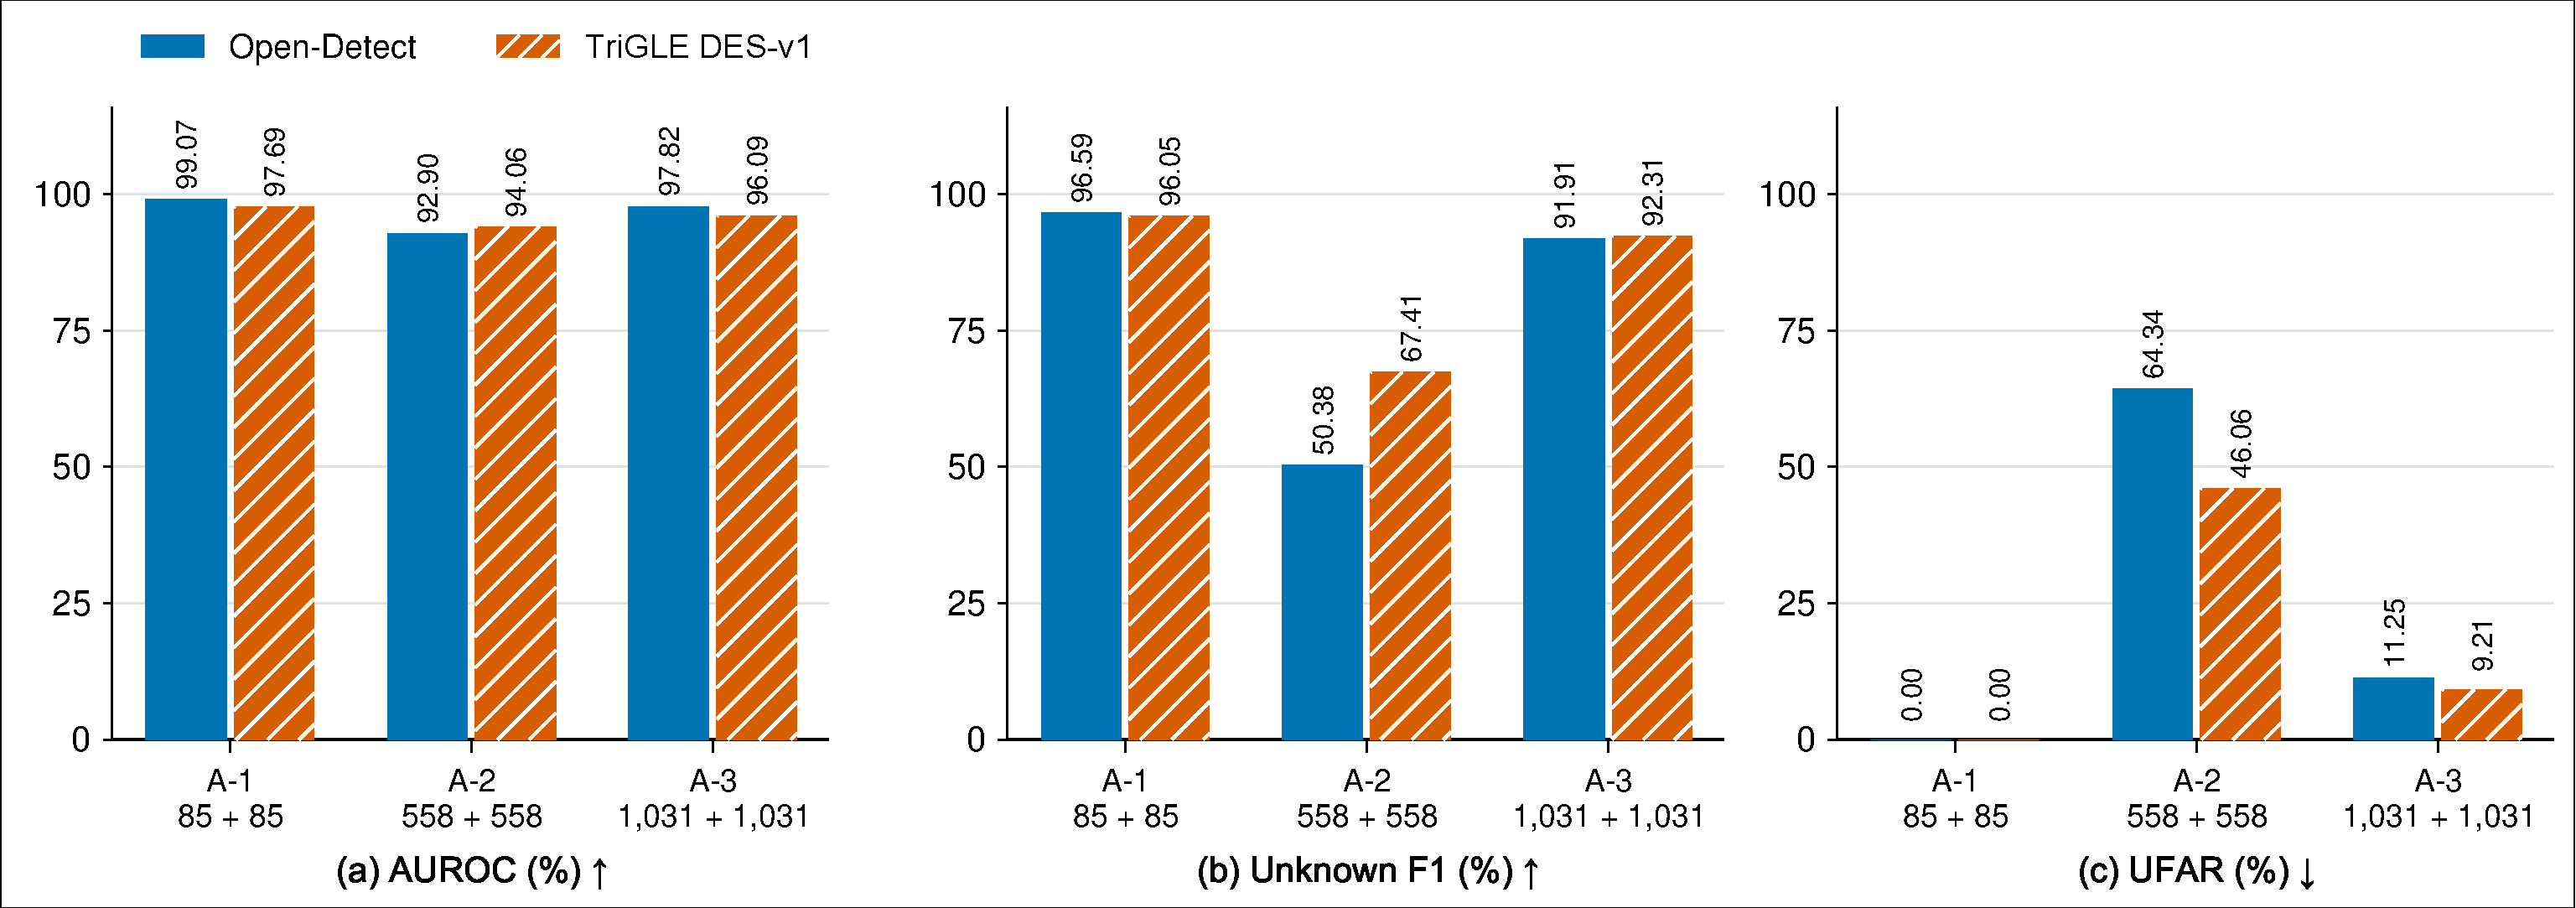
\includegraphics[width=0.96\textwidth,trim=3bp 3bp 3bp 3bp,clip,keepaspectratio]{images/suggestion3_fig4_1.pdf}
\begingroup
\renewcommand{\thefigure}{4-1}
\caption{Unknown-class detection performance under three USTC class-holdout configurations. (a) AUROC; (b) unknown-class F1; (c) UFAR.}
\label{fig:source-4-1}
\endgroup
\end{figure*}

\begin{figure*}[!t]
\centering
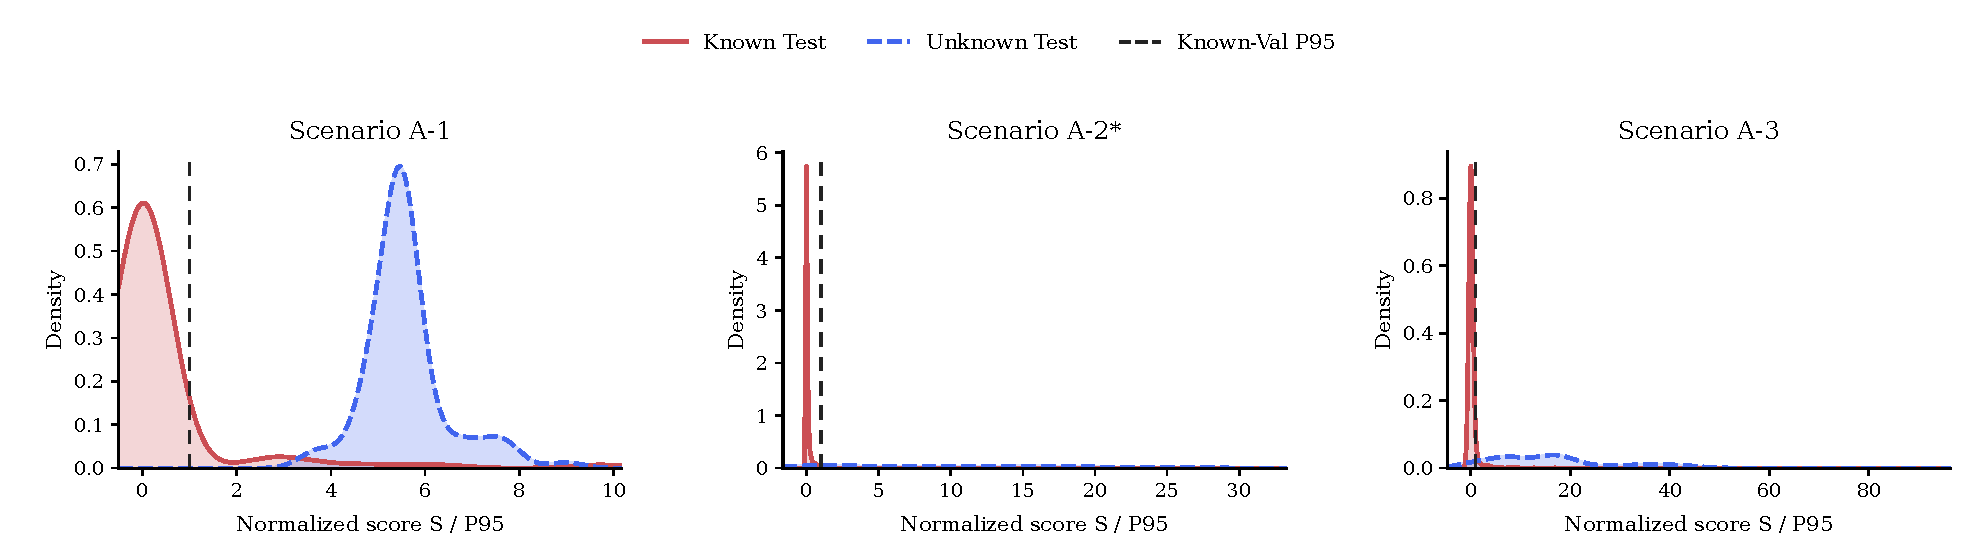
\includegraphics[width=0.98\textwidth,keepaspectratio]{images/ustc_score_distributions_normalized.pdf}
\begingroup
\renewcommand{\thefigure}{4-2}
\caption{Known and unknown score distributions in the USTC A-1, A-2, and A-3 settings.}
\label{fig:source-4-2}
\endgroup
\end{figure*}

\textbf{Class-level responses to unknown attacks.} Table~4-8 reports MSP and DES-v1 AUROC and DES-v1 AUPRC and UFAR for ten unknown CIC attacks. This comparison contrasts classification confidence with empirical support scores across attack scenarios.


\begin{table}[H]
\centering
\begingroup
\renewcommand{\thetable}{4-8}
\caption{Recognition results for ten unknown CIC attacks (\%, original test-pool proportions, P95)}\label{tab:source-8-cic}
\fontsize{7}{8.5}\selectfont
\setlength{\tabcolsep}{0pt}
\begin{tabular}{@{}>{\raggedright\arraybackslash}p{0.30\columnwidth}*{5}{>{\centering\arraybackslash}p{0.14\columnwidth}}@{}}
\hline
Unknown attack & \shortstack{Unknown\\flows} & \shortstack{MSP\\AUROC} & \shortstack{DES-v1\\AUROC} & \shortstack{DES-v1\\AUPRC} & \shortstack{DES-v1\\UFAR $\downarrow$} \\
\hline
DoS slowloris & 5,709 & 81.47 & \textbf{99.31} & 99.67 & 0.04 \\
DoS GoldenEye & 7,441 & 33.17 & \textbf{97.00} & 97.72 & 0.24 \\
DoS Hulk & 155,168 & 9.38 & \textbf{97.38} & 99.88 & 0.11 \\
FTP-Patator & 3,985 & 98.75 & \textbf{99.83} & 99.86 & 0.00 \\
SSH-Patator & 2,987 & 86.97 & \textbf{99.13} & 98.93 & 0.00 \\
Web Attack -- Brute Force & 1,364 & 91.61 & \textbf{99.57} & 99.14 & 0.00 \\
Web Attack -- XSS & 629 & 97.80 & \textbf{99.75} & 98.84 & 0.00 \\
DoS Slowhttptest & 5,096 & 85.97 & \textbf{99.34} & 99.63 & 0.14 \\
DDoS & 76,613 & 5.82 & \textbf{94.90} & 99.45 & 16.61 \\
Bot & 1,228 & 62.91 & \textbf{94.64} & 87.58 & 50.90 \\
\hline
\end{tabular}
\endgroup
\end{table}


DES-v1 achieves UFAR no greater than 0.24\% for eight of the ten unknown attacks, indicating effective rejection overall. Known FRR is 7.13\% for every attack category. For Hulk, MSP achieves only 9.38\% AUROC, whereas DES-v1 reaches 97.38\%, indicating that empirical support distance can compensate for classification-confidence failures on some unknown attacks. Bot and DDoS remain challenging, with UFAR values of 50.90\% and 16.61\%, respectively. This variation indicates that feature overlap between attack types and known classes affects rejection performance.

DDoS achieves 99.45\% AUPRC, but unknown samples account for 97.12\% of its original test pool and UFAR remains 16.61\%. Thus, under class imbalance, high AUPRC does not imply a low false acceptance rate at a fixed threshold. Rejection performance therefore requires joint assessment using ranking and threshold-dependent metrics. Together with VNAT and USTC, these results show effective overall unknown detection and recognition for most classes, while leaving room for improvement on unknown attacks whose feature distributions overlap those of known classes. We will address these difficult unknown classes in future work.

\subsection{Rejection Mechanism and Component Ablations}
\subsubsection{Roles of Global and Local Empirical Support}
To separate full-system gains from the contribution of the rejection rule, we fix the encoders, fused features $h(x)$, and classification outputs $\ell(x)$ across the four VNAT folds and change only the unknown-detection score. MSP and Energy use classification outputs. DES-v0 uses the squared distance to the nearest empirical centroid. DES-v1 incorporates the mean Euclidean distance to the 10 nearest neighbors within the nearest-centroid class. Each score independently calibrates its threshold on the known-class validation set. Table~4-9 presents the results.


\begin{table}[H]
\centering
\begingroup
\renewcommand{\thetable}{4-9}
\caption{Rejection scores on identical frozen representations (\%, equal-weight mean over four folds, original test-pool proportions, P95)}\label{tab:source-8}
\fontsize{8}{9.5}\selectfont
\setlength{\tabcolsep}{1pt}
\begin{tabular*}{\columnwidth}{@{\extracolsep{\fill}}lccccc@{}}
\hline
Rejection score & AUROC & AUPRC & Unknown F1 & UFAR & Known FRR \\
\hline
MSP & 91.83 & 96.66 & 90.55 & 14.63 & 4.93 \\
Energy & 91.73 & 96.58 & 89.96 & 15.40 & 4.87 \\
DES-v0 & 97.43 & 98.79 & 96.10 & 5.59 & 4.87 \\
\textbf{DES-v1} & \textbf{99.22} & \textbf{99.50} & \textbf{98.40} & \textbf{1.09} & \textbf{4.45} \\
\hline
\end{tabular*}
\par\smallskip\parbox{\columnwidth}{\fontsize{7}{8}\selectfont Note: DES-v0 uses empirical centroids only; DES-v1 combines global and local support. Higher AUROC, AUPRC, and Unknown F1 are better; lower UFAR and Known FRR are better.}
\endgroup
\end{table}


Local nearest-neighbor information further improves unknown detection on fixed representations. Compared with DES-v0, DES-v1 increases mean AUROC from 97.43\% to 99.22\%, reduces UFAR from 5.59\% to 1.09\%, and reduces Known FRR from 4.87\% to 4.45\%. For Remote Access, AUROC rises from 94.47\% to 98.76\%; for Communication, it rises from 98.24\% to 99.54\%. This comparison directly supports the combination of global and local empirical support in Section~III: neighborhoods of actual samples provide rejection information beyond class means. Fig.~4-4 visualizes these per-service differences.

The File Transfer fold further illustrates the trade-off between the two error rates. DES-v1 reduces Known FRR from 5.03\% to 4.61\%, while UFAR increases from 0.36\% to 0.56\%. Local support therefore primarily improves ranking across the four folds and average acceptance behavior. A specific operating point still requires joint assessment of false rejection of known services and false acceptance of unknown traffic.

\begin{figure*}[!t]
\centering
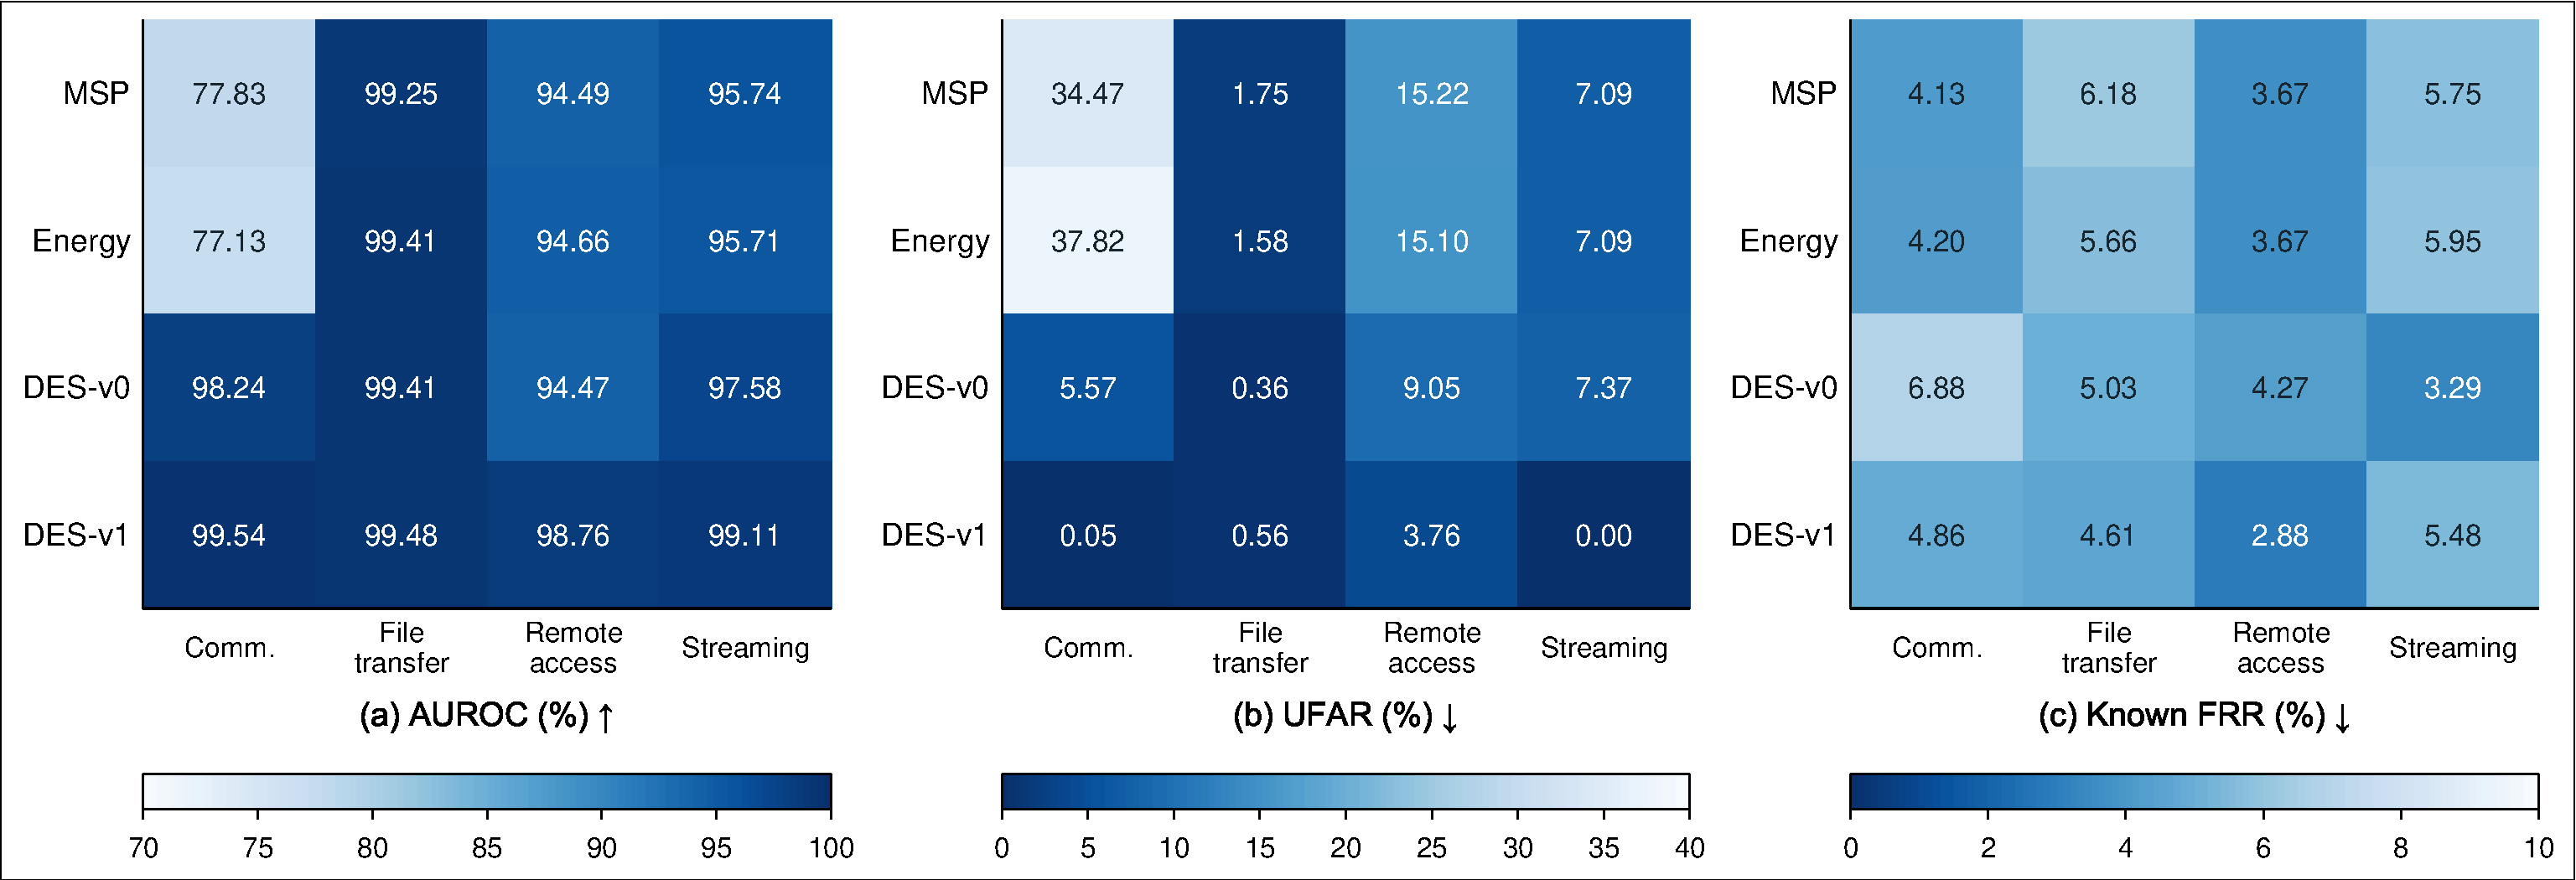
\includegraphics[width=0.88\textwidth,trim=4bp 4bp 4bp 4bp,clip,keepaspectratio]{images/Fig4_4_Reference.pdf}
\begingroup
\renewcommand{\thefigure}{4-4}
\caption{Ablation of rejection scores on identical TriGLE representations. Columns denote the four unknown services, and rows denote the four scores. The figure reports AUROC, UFAR, and Known FRR in sequence; all cells are percentages.}
\label{fig:source-4-3}
\endgroup
\end{figure*}

\subsubsection{View Contributions}
We ablate the FIG, YaTC, and TrafficFormer branches individually under the same four-fold VNAT configuration to assess each branch's contribution to the final representation. The encoders, Gaussian adapters, and normalization parameters remain frozen. All configurations retain the same fusion-head architecture and training settings for comparability. Table~4-10 reports closed-set classification and unknown-detection performance.


\begin{table}[H]
\centering
\begingroup
\renewcommand{\thetable}{4-10}
\caption{VNAT view ablations under the same configuration (\%, equal-weight mean over four folds, DES-v1, original test-pool proportions, P95)}\label{tab:source-9}
\fontsize{6.5}{8}\selectfont
\setlength{\tabcolsep}{1pt}
\begin{tabular}{@{}lcccccc@{}}
\hline
Configuration & Known Macro-F1 & AUROC & AUPRC & Unknown F1 & UFAR & Known FRR \\
\hline
TriGLE (full) & 99.87 & 99.22 & 99.50 & 98.40 & 1.09 & 4.45 \\
Without FIG & 97.08 & 97.45 & 97.37 & 97.24 & 1.41 & 3.49 \\
Without YaTC & 96.56 & 95.92 & 96.75 & 89.83 & 14.80 & 4.91 \\
Without TrafficFormer & 95.21 & 96.35 & 94.81 & 94.14 & 8.53 & 4.81 \\
\hline
\end{tabular}
\par\smallskip\parbox{\columnwidth}{\fontsize{7}{8}\selectfont Note: Higher Known Macro-F1, AUROC, AUPRC, and Unknown F1 are better; lower UFAR and Known FRR are better.}
\endgroup
\end{table}


Removing any branch degrades some key detection metrics in Table~4-10. Removing YaTC decreases unknown-class F1 from 98.40\% to 89.83\% and increases UFAR from 1.09\% to 14.80\%, indicating the importance of multilevel byte representations for separating unknown traffic from known classes. Removing TrafficFormer decreases AUPRC from 99.50\% to 94.81\% and unknown-class F1 to 94.14\%, indicating that contextual information in byte sequences complements known-class discrimination and unknown detection. Removing FIG decreases AUROC and AUPRC to 97.45\% and 97.37\%, respectively, decreases unknown-class F1 to 97.24\%, and increases UFAR to 1.41\%. These results indicate that the flow interaction graph provides structural information for traffic discrimination and unknown detection by modeling relationships between packets. Overall, the three views provide complementary information that jointly improves known-class recognition and unknown-class rejection.

\subsection{Sensitivity to the Rejection Threshold and Test Distribution}

\subsubsection{Effect of the Rejection Threshold}
The preceding results use the fixed P95 operating point. We retain the VNAT network, training support bank, and score, and additionally use P90 and P99 of the known-class validation scores to examine false acceptance and false rejection. Table~4-11 uses the existing four-fold results, with P95 remaining the primary operating point.


\begin{table}[H]
\centering
\begingroup
\renewcommand{\thetable}{4-11}
\caption{Sensitivity to validation-quantile thresholds on VNAT (\%, DES-v1, equal-weight mean over four folds, original test-pool proportions)}\label{tab:source-10}
\fontsize{7}{8.5}\selectfont
\setlength{\tabcolsep}{2pt}
\begin{tabular}{@{}cccc@{}}
\hline
Validation quantile & Unknown F1 $\uparrow$ & UFAR $\downarrow$ & Known FRR $\downarrow$ \\
\hline
P90 & 97.26 & 0.91 & 10.02 \\
P95 & 98.40 & 1.09 & 4.45 \\
P99 & 85.94 & 20.98 & 1.23 \\
\hline
\end{tabular}
\endgroup
\end{table}


The validation quantile directly controls the trade-off between acceptance of known samples and missed detection of unknown samples. P90 reduces mean UFAR to 0.91\% but increases Known FRR to 10.02\%. P99 reduces Known FRR to 1.23\% but increases UFAR to 20.98\%. A more permissive threshold increases known acceptance and may also increase missed unknown detections. All three operating points share the same score, so AUROC and AUPRC remain unchanged. Fixed-threshold error rates thus complement ranking metrics by characterizing acceptance behavior.

\subsubsection{Unknown Proportion and Class Composition}
Threshold sensitivity examines acceptance criteria under a fixed distribution, whereas mixed testing examines sample composition. From the frozen score pools for the ten CIC attacks, we draw 2,000 flows per trial and repeat the experiment using 20 deterministic seeds. With equal known and unknown proportions and equal representation of the ten unknown classes, DES-v1 achieves mean AUROC of 98.10\%, unknown-class F1 of 93.12\%, UFAR of 6.71\%, and Known FRR of 7.07\%. The model and P95 threshold remain frozen throughout.

Fig.~4-5 shows AUROC, AUPRC, UFAR, and Known FRR at five proportions of unknown traffic.

\begin{figure}[H]
\centering
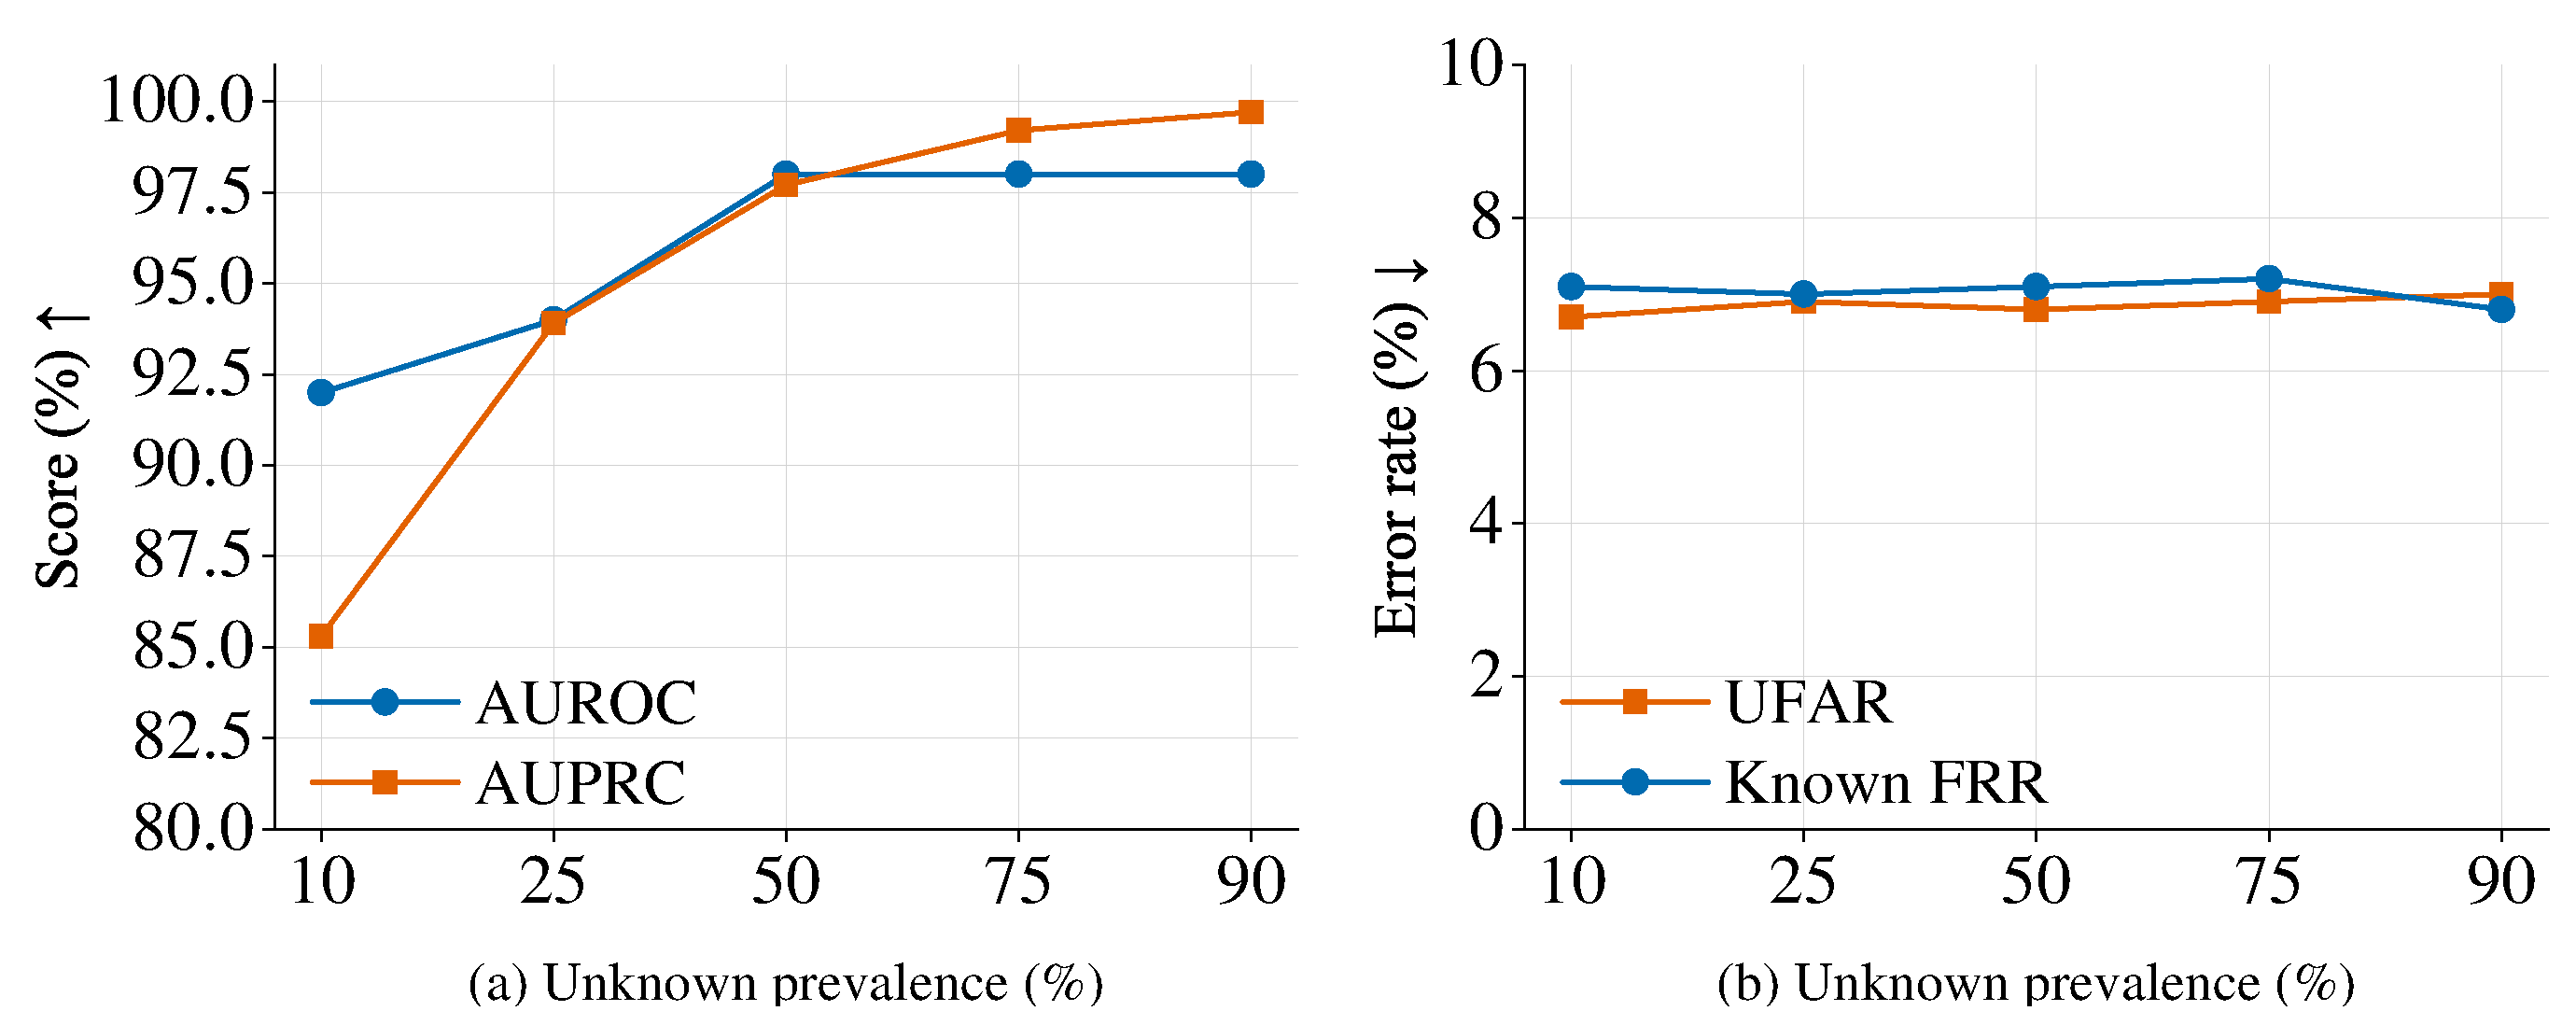
\includegraphics[width=\columnwidth,keepaspectratio]{images/suggestion2_fig4_5.pdf}
\begingroup
\renewcommand{\thefigure}{4-5}
\caption{Prevalence sensitivity across five equally spaced settings. (a) AUROC and AUPRC. (b) UFAR and Known FRR.}
\label{fig:source-4-4}
\endgroup
\end{figure}

Ranking performance and conditional error rates remain relatively stable as the proportion of unknown samples changes. With the ten unknown classes balanced internally and the known-to-unknown ratio varying from 9:1 to 1:9, Fig.~4-5 shows AUROC ranging from approximately 92.0\% to 98.0\% and UFAR from approximately 6.7\% to 7.0\%. AUPRC increases from approximately 85.3\% to 99.7\% as the unknown proportion rises. At a fixed 1:1 ratio, mixing only Bot and DDoS attack samples increases UFAR to 33.84\%. Changes in the composition of normal traffic and PortScan also affect Known FRR. Together with the per-attack results, these findings indicate that the detector is more sensitive to unknown-class composition than to the overall proportion of unknown samples.

\section{Conclusion}
The experiments show that TriGLE classifies known traffic and rejects many unknown services and attacks under the stated protocols.\par\smallskip
\textbf{Limitations:} We validate the proposed method on multiple public datasets and under different unknown-class holdout settings, but dataset provenance and traffic distributions constrain the experiments. The datasets differ in capture environments, application types, and traffic composition. Unknown-class feature distributions also strongly affect rejection performance. The model still falsely accepts some unknown traffic whose features resemble those of known classes.

\textbf{Future work:} We will expand dataset and experimental coverage through cross-dataset and cross-network-environment generalization tests to assess adaptation to different traffic distributions. To address feature overlap between unknown and known classes, we will investigate more effective local feature modeling and rejection strategies for difficult unknown classes. We will also examine the effects of packet padding, segmentation, and traffic perturbations on multiview representations and explore detection methods that depend less on raw bytes to improve robustness in complex network environments.
